% ============================================================================
%  DOCUMENTO PRINCIPAL
%  ----------------------------------------------------------------------------
%  Aquí SOLO se integran los módulos. No se escribe contenido ni formato aquí.
%
%  Regla de oro del proyecto:
%    - formato/preambulo.sty  -> toda la configuración y paquetes (APA + Arial)
%    - formato/portada.tex    -> portada (datos institucionales)
%    - contenido/*.tex        -> el contenido real del informe
%    - anexos/*.tex           -> material complementario
%
%  Para compilar (desde docs/latex/):
%    pdflatex main && bibtex main && pdflatex main && pdflatex main
%  o directamente: latexmk -pdf main.tex
% ============================================================================

\documentclass[12pt,letterpaper]{article}

% --- Carga de la configuración de formato (APA + Arial) ---------------------
\usepackage{formato/preambulo}

% ============================================================================
%  DATOS DEL DOCUMENTO  (editar aquí)
%  Los valores entre corchetes [ ] son marcadores que debes reemplazar.
% ============================================================================
\newcommand{\tituloDocumento}{Desarrollo de un Sistema Web y M\'ovil para la
  Visualizaci\'on Interactiva de Escenarios Deportivos a Nivel Nacional}
\newcommand{\nombreApp}{DeporteYa}              % nombre provisional de la aplicación
\newcommand{\equipo}{Sudoers}
\newcommand{\integrantes}{%
  Angel Gabriel Rojas Hinojosa \par
  Joaquin Alessandro Felipez Rojas \par
  Nicolas Sebastian Reguerin Meneses \par
  David Willy Cruz Huanca}
\newcommand{\universidad}{Universidad Privada Domingo Savio}
\newcommand{\facultad}{Facultad de Ingenier\'ia}
\newcommand{\carrera}{Ingenier\'ia en Sistemas}
\newcommand{\asignatura}{Aplicaciones M\'oviles I}
\newcommand{\docente}{Vladimir Wilmar Rojas Condori}
\newcommand{\ciudad}{Cochabamba--Bolivia}
\newcommand{\fechaEntrega}{\today}

\begin{document}

% --- Portada ----------------------------------------------------------------
% ============================================================================
%  PORTADA  (formato APA, página de título)
%  ----------------------------------------------------------------------------
%  Los datos provienen de las macros definidas en main.tex. No editar aquí.
% ============================================================================

\begin{titlepage}
  \thispagestyle{empty}
  \begin{center}
    {\LARGE\bfseries \universidad \\[4pt]}

    \vspace{0.4cm}
    {\large \facultad \\[4pt]}
    {\large \carrera}

    \vspace{3.5cm}
    \rule{\linewidth}{1.2pt}
    \vspace{1cm}

    {\Large\bfseries \tituloDocumento}

    \vspace{1cm}
    \rule{\linewidth}{1.2pt}

    \vspace{3.5cm}
    {\large\bfseries Autor: \autor}

    \vspace{1.5cm}
    {\large Asignatura: \asignatura \\[4pt]}
    {\large Docente: \docente}

    \vspace{2.5cm}
    {\large \fechaEntrega}
  \end{center}
\end{titlepage}


% --- Resumen y palabras clave ----------------------------------------------
% ============================================================================
%  RESUMEN
% ============================================================================

\begin{abstract}
\noindent
\textbf{Objetivo:} Desarrollar e integrar un m\'odulo de inscripci\'on a
eventos deportivos en la aplicaci\'on m\'ovil \nombreApp{}, que permita a los
usuarios registrarse, cancelar inscripciones y consultar su estado de
inscripci\'on desde la interfaz de la aplicaci\'on.

\medskip
\noindent
\textbf{Metodolog\'ia:} Se sigui\'o un proceso de an\'alisis de necesidades,
dise\~no de interfaz, implementaci\'on de backend (Supabase/PostgreSQL),
desarrollo de componentes React Native con Expo, y pruebas de integraci\'on.
El m\'odulo se bas\'o en la arquitectura existente del proyecto, reutilizando
hooks de React Query, el sistema de dise\~no de colores y los patrones de
navegaci\'on con Expo Router.

\medskip
\noindent
\textbf{Resultados:} Se implement\'o una tabla \texttt{event\_registrations}
con pol\'iticas RLS granulares, hooks personalizados para las operaciones
CRUD, un componente de bot\'on de inscci\'on con estados visuales, y una
secci\'on de ``Mis inscripciones'' en el perfil del usuario. El m\'odulo
cumple con los requisitos de validaci\'on, manejo de errores, persistencia
en la nube e integraci\'on con la aplicaci\'on existente.

\medskip
\noindent
\textbf{Palabras clave:} inscripci\'on a eventos, React Native, Expo,
Supabase, PostgreSQL, CRUD, RLS, aplicaciones m\'oviles.
\end{abstract}


% --- Índices ----------------------------------------------------------------
\newpage
\tableofcontents
\newpage
\listoftables
\newpage
\listoffigures

% ============================================================================
%  CONTENIDO  (un capítulo con su carátula y un archivo por sección)
% ============================================================================

% --- CAPÍTULO I: INTRODUCCIÓN ------------------------------------------------
\caratulaCapitulo{CAP\'ITULO I}{INTRODUCCI\'ON}
% ============================================================================
%  SECCIÓN 1.1: ANTECEDENTES
% ============================================================================

\section{Antecedentes}

Los antecedentes consisten en la presentaci\'on de la informaci\'on m\'as
relevante y directamente relacionada con el tema del proyecto. Su estudio
garantiza que el trabajo parta del punto m\'as actual de la tem\'atica en
cuesti\'on. Para su elaboraci\'on se emplean los m\'etodos hist\'orico l\'ogico y
deductivo, partiendo de elementos generales, como el desarrollo de la
infraestructura deportiva del pa\'is, hasta llegar a los aspectos espec\'ificos
relacionados con la difusi\'on de la oferta deportiva y el uso de tecnolog\'ias de
informaci\'on en este \'ambito.

\subsection{Antecedentes hist\'oricos}

El deporte y su infraestructura han sido parte de la vida social del pa\'is
desde comienzos del siglo XX. Escenarios emblem\'aticos como el Estadio Hernando
Siles de La Paz, inaugurado en 1930, el Estadio F\'elix Capriles de
Cochabamba y el Estadio Ram\'on Tahuichi Aguilera de Santa Cruz de la Sierra
han sido, durante d\'ecadas, los centros de la pr\'actica deportiva y del
encuentro social de las comunidades. Con el paso del tiempo, la oferta de
recintos se ha diversificado: estadios, coliseos cerrados, canchas de
baloncesto y voleibol, frontones, piscinas, pistas de atletismo y complejos
polideportivos distribuidos en los nueve departamentos del pa\'is.

Sin embargo, la informaci\'on sobre estos espacios siempre ha estado
fragmentada y ha dependido de la difusi\'on que cada recinto realiza de manera
individual mediante medios impresos, radiales, televisivos o redes sociales.
Esta situaci\'on hist\'orica explica que, a pesar de contar con una
infraestructura deportiva considerable, la poblaci\'on no disponga de un medio
unificado para conocerla.

\subsection{Antecedentes tem\'aticos}

A nivel internacional existen plataformas consolidadas que integran
informaci\'on georreferenciada sobre espacios deportivos, de recreaci\'on y de
esparcimiento, tales como directorios de instalaciones deportivas, sistemas
de reserva de canchas y aplicaciones de mapas que combinan cat\'alogo,
fotograf\'ias, horarios y eventos. Estas soluciones han demostrado que la
centralizaci\'on de la informaci\'on incrementa la visibilidad de los recintos,
favorece el uso de la infraestructura existente y facilita la toma de
decisiones de los usuarios \citep{longley2015, pressman2010}.

No obstante, la mayor\'ia de estas plataformas responden a contextos de
pa\'ises desarrollados y no se adaptan a las particularidades del medio
nacional, donde la informaci\'on deportiva es escasa y poco estructurada. El
tema ha sido abordado de forma limitada en la literatura local, y los pocos
intentos de digitalizaci\'on se concentran en recintos individuales o en
instituciones espec\'ificas, sin una visi\'on integradora a nivel pa\'is.

\subsection{Antecedentes institucionales}

El proyecto se enmarca en el \'ambito de las instituciones deportivas y
educativas del pa\'is. Los escenarios deportivos, tanto p\'ublicos como
privados, as\'i como las federaciones deportivas, los clubes y las
direcciones municipales de deportes, constituyen la poblaci\'on institucional
objetivo del sistema. Estas instituciones comparten la necesidad com\'un de
visibilizar su oferta deportiva, pero carecen de herramientas tecnol\'ogicas
adecuadas para hacerlo, lo que justifica la propuesta de una plataforma
centralizada.

\subsection{Investigaciones previas}

Diversos estudios en el \'ambito de los sistemas de informaci\'on geogr\'afica
(SIG) aplicados a servicios urbanos han demostrado que la visualizaci\'on
cartogr\'afica de la infraestructura mejora la accesibilidad a la informaci\'on
y apoya la planificaci\'on de pol\'iticas p\'ublicas \citep{longley2015}.
Trabajos similares, orientados al turismo y a la recreaci\'on, han utilizado
mapas interactivos y bases de datos centralizadas con resultados favorables
en t\'erminos de difusi\'on y participaci\'on de los usuarios. Estos hallazgos
orientan la metodolog\'ia y el dise\~no de la presente propuesta.

\subsection{Estad\'isticas consultadas}

Las fuentes estad\'isticas consultadas reflejan una baja participaci\'on de la
poblaci\'on en la actividad f\'isica y deportiva, atribuida en gran medida a la
falta de informaci\'on sobre la oferta disponible. Encuestas de h\'abitos
deportivos se\~nalan que el desconocimiento de la ubicaci\'on de los escenarios,
de las disciplinas que albergan y de los horarios de uso es una de las
principales barreras para la pr\'actica deportiva. Estas cifras respaldan la
pertinencia de la propuesta y sirven de base para la definici\'on de los
indicadores del proyecto \citep{hernandez2014}.

\begin{figure}[H]
  \centering
  
\includegraphics[width=0.62\linewidth]{escenarios-deportivos.jpeg}
  \caption{Imagen ilustrativa de los escenarios deportivos del pa\'is}
  \label{fig:infraestructura-deportiva}
\end{figure}

\textbf{FUENTE:} Elaboraci\'on propia en base a la revisi\'on documental del
sector deportivo.

\section{Contextualizaci\'on de la problem\'atica}
% TODO: Redactar el contexto del sector cultural, escenarios y teatros a nivel
% nacional; estado actual de la digitalizaci\'on y difusi\'on de la oferta cultural.

% ============================================================================
%  SECCIÓN 1.3: PLANTEAMIENTO DEL PROBLEMA
% ============================================================================

\section{Planteamiento del problema}

\subsection{Situaci\'on problem\'atica}

A partir de lo expuesto en los antecedentes, la \textbf{situaci\'on
problem\'atica} se puede establecer de la siguiente manera: la informaci\'on
sobre los escenarios deportivos a nivel nacional se encuentra dispersa,
desactualizada y sin un medio unificado de consulta, lo que impide que la
poblaci\'on conozca, localice y acceda a la oferta deportiva y limita la
visibilidad de los propios recintos.

Las causas de esta situaci\'on son la ausencia de un registro centralizado de
escenarios deportivos, la escasa digitalizaci\'on del sector y la falta de
herramientas de visualizaci\'on interactiva adaptadas al contexto nacional.
Como efecto, se observa una baja asistencia a los eventos deportivos, la
subutilizaci\'on de la infraestructura existente y el desaprovechamiento de
las oportunidades econ\'omicas y sociales que el deporte genera. Como se\~nala
\citet{arias2012}, el problema constituye el punto de partida de toda
investigaci\'on y surge cuando se identifica una situaci\'on de carencia o una
necesidad no satisfecha, tal como ocurre en este caso.

\subsection{Objeto de estudio}

El objeto de estudio del presente proyecto es el \textbf{proceso de difusi\'on
y acceso a la informaci\'on sobre los escenarios deportivos a nivel
nacional}, incluyendo los mecanismos de registro, actualizaci\'on y consulta
de los datos de cada recinto. Se justifica su estudio porque la mejora de
este proceso, mediante una soluci\'on tecnol\'ogica, permite incrementar la
pr\'actica deportiva de la poblaci\'on, optimizar la gesti\'on de los espacios
deportivos y favorecer la toma de decisiones de las entidades
administradoras.

\subsection{Estudio de soluciones}

Se analizaron soluciones contempor\'aneas aplicadas en contextos similares,
tanto nacionales como internacionales, con el fin de identificar las
pr\'acticas m\'as efectivas. La siguiente tabla presenta la valoraci\'on de los
casos de estudio analizados:

\begin{table}[H]
  \centering
  \caption{Valoraci\'on de soluciones existentes}
  \label{tab:estudio-soluciones}
  \begin{tablaAPA}
    \begin{tabular}{@{}p{4.2cm}p{3.0cm}p{4.2cm}p{3.6cm}@{}}
      \toprule
      \textbf{Casos de estudio} & \textbf{Problema} &
      \textbf{Soluci\'on aplicada} & \textbf{Valoraci\'on} \\
      \midrule
      Aplicaciones internacionales de mapas deportivos &
      Informaci\'on deportiva dispersa &
      Sistema web y m\'ovil con mapa de instalaciones y reservas &
      Soluci\'on fiable y escalable; potencial referencia para el medio
      nacional \\
      \addlinespace
      Directorios municipales de espacios de recreaci\'on &
      Falta de visibilidad de los recintos &
      Plataforma centralizada con fichas de recintos y programaci\'on &
      Soluci\'on efectiva; validada por el p\'ublico y los gestores \\
      \addlinespace
      Redes sociales de escenarios locales, Bolivia &
      Difusi\'on fragmentada por recinto &
      Publicaci\'on individual en redes sociales &
      Soluci\'on parcial: no integra la oferta a nivel nacional \\
      \bottomrule
    \end{tabular}
  \end{tablaAPA}
\end{table}

\textbf{FUENTE:} Elaboraci\'on propia en base a la revisi\'on documental de
plataformas deportivas.

\subsection{\'Arbol de causas y efectos}

Para profundizar el an\'alisis de la situaci\'on problem\'atica se emplea la
t\'ecnica del \'arbol de problemas o \'arbol de causas y efectos. En este
diagrama, la parte central (tronco) representa el problema central; la parte
superior agrupa los efectos del problema y la parte inferior re\'une las
causas que lo originan \citep{arias2012}.

\begin{figure}[H]
  \centering
  \begin{tikzpicture}[
      node distance=1.2cm and 0.5cm,
      base/.style={
        rectangle, draw, thick, rounded corners=1.5mm, 
        minimum height=1.3cm, align=center, 
        font=\small, text width=4.5cm, inner sep=2mm
      },
      efecto/.style={base, fill=red!10, draw=red!70!black},
      problema/.style={base, fill=orange!15, draw=orange!80!black, text width=5.5cm, font=\small\bfseries},
      causa/.style={base, fill=blue!10, draw=blue!70!black},
      flecha/.style={-Stealth, thick, draw=black!60, line width=1.2pt}
    ]

    % 1. Tronco: problema central (Centro)
    \node[problema] (p) {INFORMACI\'ON SOBRE ESCENARIOS DEPORTIVOS DISPERSA Y SIN VISUALIZACI\'ON INTERACTIVA};

    % 2. Efectos del problema (Parte superior, ramificados)
    \node[efecto, above=1.5cm of p] (e2) {Subutilizaci\'on de la infraestructura deportiva existente};
    \node[efecto, left=0.5cm of e2] (e1) {Baja asistencia del p\'ublico a los eventos deportivos};
    \node[efecto, right=0.5cm of e2] (e3) {Dificultad para la promoci\'on del deporte y la actividad f\'isica};

    % 3. Causas del problema (Parte inferior, ramificadas)
    \node[causa, below=1.5cm of p] (c2) {Escasa digitalizaci\'on del sector deportivo};
    \node[causa, left=0.5cm of c2] (c1) {Ausencia de un registro centralizado de escenarios deportivos};
    \node[causa, right=0.5cm of c2] (c3) {Falta de herramientas de visualizaci\'on interactiva};

    % 4. Flechas (Causas -> Problema -> Efectos)
    
    % De las causas al problema
    \draw[flecha] (c1.north) -- (p.south);
    \draw[flecha] (c2.north) -- (p.south);
    \draw[flecha] (c3.north) -- (p.south);

    % Del problema a los efectos
    \draw[flecha] (p.north) -- (e1.south);
    \draw[flecha] (p.north) -- (e2.south);
    \draw[flecha] (p.north) -- (e3.south);

  \end{tikzpicture}
  \caption{\'Arbol de causas y efectos del problema identificado}
  \label{fig:arbol-causas-efectos}
\end{figure}

Las causas detectadas se han depurado agrupando aquellas que se encuentran
relacionadas entre s\'i y descartando las que se repet\'ian o que no afectaban
directamente a la poblaci\'on en la que se llevar\'a a cabo la investigaci\'on.
El an\'alisis causa--efecto expuesto permite pasar de la identificaci\'on del
problema a su formulaci\'on, que se presenta en la siguiente secci\'on.

% ============================================================================
%  SECCIÓN 1.4: FORMULACIÓN DEL PROBLEMA
% ============================================================================

\section{Formulaci\'on del problema}

La forma m\'as habitual de plantear un problema de investigaci\'on es mediante
una interrogaci\'on, aunque tambi\'en puede expresarse como un enunciado que
describa exactamente cu\'al es el problema que se pretende resolver. Para su
formulaci\'on se han considerado la magnitud, la trascendencia y la viabilidad
del problema, as\'i como su car\'acter factible y contrastable
\citep{arias2012}.

\subsection{Enunciado del problema}

El problema identificado se puede enunciar de la siguiente manera:

\begin{quote}
\textit{Insuficiente acceso de la ciudadan\'ia a informaci\'on confiable,
actualizada y georreferenciada sobre los escenarios deportivos del pa\'is, lo
que limita la pr\'actica deportiva y el aprovechamiento de la
infraestructura deportiva nacional.}
\end{quote}

El problema es factible de resolver porque la informaci\'on necesaria existe y
se genera de forma continua; lo que falta es un medio digital, centralizado e
interactivo que la organice y la ponga a disposici\'on de los usuarios. Es
contrastable, pues los resultados de la soluci\'on podr\'an verificarse mediante
indicadores de uso, cobertura y satisfacci\'on de los usuarios.

\subsection{Pregunta de investigaci\'on}

A partir del an\'alisis anterior, el problema se formula mediante la siguiente
pregunta de investigaci\'on:

\begin{quote}
\textit{¿C\'omo podr\'ia un sistema web y una aplicaci\'on m\'ovil contribuir a la
visualizaci\'on interactiva de los escenarios deportivos a nivel nacional,
facilitando a la ciudadan\'ia el acceso a informaci\'on confiable y actualizada
sobre su ubicaci\'on, sus caracter\'isticas y su oferta deportiva?}
\end{quote}

La respuesta a esta pregunta orienta el planteamiento de los objetivos de la
investigaci\'on, que constituyen el punto de referencia del estudio y se
desarrollan en la siguiente secci\'on.

% ============================================================================
%  SECCIÓN 1.5: OBJETIVOS DE LA INVESTIGACIÓN
% ============================================================================

\section{Objetivos de la investigaci\'on}

Los objetivos de la investigaci\'on son el punto de referencia del estudio, ya
que orientan las acciones necesarias para alcanzar los resultados que se
pretenden lograr con el desarrollo del proyecto \citep{arias2012}. Deben
redactarse con verbos en infinitivo que implican acciones concretas que se
ejecutan durante la investigaci\'on.

\subsection{Objetivo general}

El objetivo general constituye el prop\'osito general que se persigue con el
proceso de investigaci\'on. Es un enunciado claro y preciso de la meta global,
expresado en t\'erminos cualitativos:

\begin{quote}
\textbf{Desarrollar} un sistema web y m\'ovil para la visualizaci\'on interactiva
de escenarios deportivos a nivel nacional que facilite a la ciudadan\'ia la
localizaci\'on y el acceso a informaci\'on confiable y actualizada sobre la
infraestructura deportiva del pa\'is.
\end{quote}

\subsection{Objetivos espec\'ificos}

Los objetivos espec\'ificos constituyen los prop\'ositos particulares mediante los
cuales se puede lograr el objetivo general e indican lo que se pretende
realizar en cada una de las etapas del proyecto. Para el presente proyecto se
han definido los siguientes objetivos espec\'ificos:

\begin{enumerate}
  \item \textbf{Diagnosticar} la situaci\'on actual de la difusi\'on y el acceso
    a la informaci\'on de los escenarios deportivos a nivel nacional, mediante
    t\'ecnicas de recolecci\'on de datos como entrevistas y encuestas
    \citep{hernandez2014}, a fin de fundamentar los requerimientos del
    sistema.

  \item \textbf{Identificar y documentar} los requerimientos funcionales y no
    funcionales del sistema web y m\'ovil, siguiendo las buenas pr\'acticas de la
    ingenier\'ia de requerimientos \citep{sommerville2011}.

  \item \textbf{Dise\~nar} la arquitectura del sistema, incluyendo el modelo de
    datos, la estructura de m\'odulos y la interfaz de usuario, mediante
    diagramas y wireframes de baja fidelidad.

  \item \textbf{Desarrollar} el m\'odulo de visualizaci\'on interactiva basado en
    mapas georreferenciados, que permita ubicar los escenarios deportivos y
    consultar su informaci\'on de manera intuitiva.

  \item \textbf{Implementar} la aplicaci\'on m\'ovil multiplataforma y el sistema
    web, integrando las funcionalidades definidas en el alcance del producto
    m\'inimo viable.

  \item \textbf{Evaluar} la usabilidad, el rendimiento y la satisfacci\'on de los
    usuarios con el sistema desarrollado, aplicando pruebas funcionales y
    cuestionarios, con el prop\'osito de validar el cumplimiento de los
    objetivos planteados.
\end{enumerate}

% ============================================================================
%  SECCIÓN 1.6: DEFINICIÓN DE VARIABLES
% ============================================================================

\section{Definici\'on de variables}

La concreci\'on de los aspectos de la realidad o del problema a los que se
dirige la atenci\'on se realiza definiendo las variables. Una variable es un
aspecto de la realidad que cambia en distintas situaciones y para diferentes
objetivos y sujetos; las variables permiten agrupar, diferenciar, ordenar,
distribuir y relacionar los elementos de la realidad \citep{hernandez2014}.
Las variables no est\'an dadas de antemano, sino que hay que elaborarlas,
siendo en un principio conceptos generales que se concretan para darles
significado.

La variable es una determinada caracter\'istica o propiedad del objeto de
estudio a la cual se observa y/o cuantifica en la investigaci\'on. Para el
presente proyecto se han identificado las variables que se presentan en la
siguiente tabla, con su definici\'on conceptual, sus dimensiones, sus
indicadores y los instrumentos de recolecci\'on de datos que permitir\'an
medirlas.

\begin{table}[H]
  \centering
  \caption{Operacionalizaci\'on de las variables de la investigaci\'on}
  \label{tab:variables}
  \contenidoConFuente{%
    \begin{tablaAPA}
      \begin{tabular}{@{}p{2.3cm}p{3.5cm}p{2.8cm}p{3.8cm}p{2.3cm}@{}}
        \toprule
        \textbf{Variable} & \textbf{Definici\'on conceptual} &
        \textbf{Dimensiones} & \textbf{Indicadores} &
        \textbf{Instrumentos} \\
        \midrule
        Acceso a la informaci\'on deportiva &
        Facilidad con la que el p\'ublico obtiene informaci\'on sobre la oferta
        deportiva disponible &
        Nivel de dificultad; tiempo de b\'usqueda; canales utilizados &
        I1. Porcentaje de personas que desconoce la oferta deportiva de su
        ciudad; I2. tiempo promedio de b\'usqueda &
        Encuesta \\
        \addlinespace
        Visualizaci\'on interactiva &
        Representaci\'on gr\'afica e interactiva de la informaci\'on de los
        escenarios &
        Usabilidad del mapa; utilidad de los filtros &
        I1. Usabilidad percibida (escala); I2. tasa de uso del mapa
        interactivo &
        Encuesta, gu\'ia de observaci\'on \\
        \addlinespace
        Cobertura del sistema &
        N\'umero y distribuci\'on de los escenarios registrados en la plataforma &
        Cantidad de recintos; distribuci\'on geogr\'afica &
        I1. Escenarios registrados (total); I2. departamentos cubiertos &
        Revisi\'on documental, base de datos del sistema \\
        \bottomrule
      \end{tabular}
    \end{tablaAPA}%
  }{Elaboraci\'on propia en base a \citet{hernandez2014}.}
\end{table}

% ============================================================================
%  SECCIÓN 1.7: DELIMITACIÓN
% ============================================================================

\section{Delimitaci\'on}

La delimitaci\'on, entendida como la acci\'on y efecto de delimitar, hace
referencia a determinar las caracter\'isticas esenciales del contexto y del
objeto de estudio. En el proyecto de grado, la delimitaci\'on del contexto y del
objeto mismo de estudio es primordial, pues permite situar el problema y las
razones del mismo en el contexto especificado \citep{arias2012}.

\subsection{L\'imite temporal}

El proyecto se desarrollar\'a durante la gesti\'on acad\'emica correspondiente a
la asignatura de Aplicaciones M\'oviles I, en el marco del aprendizaje basado en
proyectos (ABP), con una duraci\'on estimada de seis meses, comprendidos entre
agosto de 2026 y enero de 2027. Las actividades se distribuyen en un
cronograma de 16 semanas organizadas en cinco fases: an\'alisis, dise\~no,
desarrollo, pruebas y cierre, tal como se detalla en el anexo correspondiente.

\subsection{L\'imite geogr\'afico}

El \'ambito geogr\'afico del proyecto es el territorio nacional, con \'enfasis en
los escenarios deportivos de las principales ciudades del pa\'is. La
informaci\'on se incorporar\'a de forma progresiva, comenzando por un piloto de
validaci\'on en las ciudades de La Paz, Cochabamba y Santa Cruz de la Sierra,
donde se concentra la mayor oferta de infraestructura deportiva del pa\'is.

\subsection{Otros l\'imites del proyecto}

El proyecto se limita a la visualizaci\'on interactiva y a la difusi\'on de
informaci\'on sobre los escenarios deportivos. Quedan fuera del alcance los
procesos de reserva, alquiler y pago en l\'inea, as\'i como la gesti\'on
administrativa interna de los escenarios, que podr\'an ser considerados en
avances futuros.

% ============================================================================
%  SECCIÓN 1.8: JUSTIFICACIÓN
% ============================================================================

\section{Justificaci\'on}

La realizaci\'on de este proyecto se justifica por la importancia de acercar la
infraestructura deportiva del pa\'is a la poblaci\'on mediante el uso de
tecnolog\'ias de informaci\'on accesibles, masivas y de bajo costo. Justificar es
exponer los motivos que ameritan realizar la investigaci\'on, respondiendo a
las preguntas de por qu\'e es importante su realizaci\'on y para qu\'e se realiza
\citep{arias2012}. En ese sentido, el proyecto aporta desde las dimensiones
social, econ\'omica, t\'ecnica, cient\'ifica y metodol\'ogica.

\subsection{Justificaci\'on social}

El proyecto beneficiar\'a directamente a la ciudadan\'ia al facilitar el acceso a
la informaci\'on sobre los escenarios deportivos, promoviendo la pr\'actica del
deporte y la actividad f\'isica como factores de salud, inclusi\'on y convivencia
social. Al visibilizar la oferta deportiva existente, se contribuye a reducir
las barreras de acceso y a fomentar h\'abitos de vida saludable en la
poblaci\'on, en particular en j\'ovenes y ni\~nos. Asimismo, se favorece la
participaci\'on de la comunidad en los eventos deportivos que se organizan en
cada regi\'on, fortaleciendo el tejido social.

\subsection{Justificaci\'on econ\'omica}

Desde el punto de vista econ\'omico, el proyecto permite optimizar el uso de la
infraestructura deportiva existente, cuya subutilizaci\'on representa una
p\'erdida de recursos para las entidades administradoras. Al dar visibilidad a
los escenarios, se incrementan las posibilidades de uso, alquiler y
organizaci\'on de eventos, generando ingresos para los administradores y
dinamizando la econom\'ia local vinculada al deporte. Adem\'as, el desarrollo de
una soluci\'on multiplataforma con herramientas de c\'odigo abierto y servicios
en la nube de bajo costo hace viable el proyecto con una inversi\'on m\'inima.

\subsection{Justificaci\'on t\'ecnica}

El proyecto aprovecha tecnolog\'ias maduras y ampliamente difundidas para el
desarrollo de aplicaciones web y m\'oviles, sistemas de informaci\'on geogr\'afica
y mapas interactivos \citep{longley2015, pressman2010}. Estas tecnolog\'ias han
sido validadas en soluciones similares de otros sectores y permiten construir
una aplicaci\'on multiplataforma (iOS y Android) con un \'unico c\'odigo base,
reduciendo costos y tiempos de desarrollo. La soluci\'on propuesta representa
una innovaci\'on en el \'ambito deportivo nacional, donde no existe actualmente un
sistema equivalente de acceso p\'ublico.

\subsection{Justificaci\'on cient\'ifica}

Los argumentos cient\'ificos que sustentan la realizaci\'on del proyecto se
fundamentan en el cuerpo te\'orico de la ingenier\'ia de software, los sistemas
de informaci\'on geogr\'afica y la metodolog\'ia de la investigaci\'on
\citep{sommerville2011, longley2015, hernandez2014}. El proyecto aplica
principios establecidos de an\'alisis y dise\~no de sistemas, usabilidad y
calidad de software, y genera nuevo conocimiento sobre la aplicaci\'on de estas
herramientas al \'ambito de la difusi\'on de la infraestructura deportiva,
obteniendo procedimientos que permiten un acercamiento eficaz al objeto de
estudio.

\subsection{Justificaci\'on metodol\'ogica}

El proyecto seguir\'a un enfoque de desarrollo \'agil e iterativo, acorde con las
buenas pr\'acticas de la ingenier\'ia de software \citep{sommerville2011,
larman2004}. La definici\'on del producto m\'inimo viable permite validar la
propuesta con usuarios reales en etapas tempranas y mejorar de forma
continua, aplicando metodolog\'ias que podr\'an servir de referencia para
proyectos similares de digitalizaci\'on de la informaci\'on deportiva.

\subsection{An\'alisis de viabilidad}

De acuerdo con la gu\'ia del avance, se analiza la viabilidad del proyecto
considerando el tiempo disponible, la cantidad de integrantes, los
conocimientos actuales, las tecnolog\'ias disponibles y la complejidad de la
soluci\'on:

\begin{itemize}
  \item Tiempo: el proyecto se desarrollar\'a durante la gesti\'on
    acad\'emica, con un cronograma de 16 semanas distribuidas en cinco fases
    (an\'alisis, dise\'no, desarrollo, pruebas y cierre).
  \item Recursos humanos: el equipo est\'a conformado por un m\'aximo de
    seis integrantes con roles definidos (l\'ider, analista, dise\'nador UI/UX,
    desarrollador y gestor de documentaci\'on).
  \item Conocimientos: las tecnolog\'ias propuestas (React Native,
    Expo, Node.js, PostgreSQL y Leaflet) se alinean con los contenidos de la
    asignatura y con las competencias del equipo.
  \item Tecnolog\'ias disponibles: se emplean herramientas de c\'odigo
    abierto y servicios en la nube con planes gratuitos, sin requerir
    inversi\'on econ\'omica significativa.
  \item Complejidad: el alcance se limita a dos o tres perfiles de
    usuario y entre cinco y ocho funcionalidades principales, definidas en el
    producto m\'inimo viable.
\end{itemize}

En consecuencia, el proyecto es viable: el problema est\'a claramente
definido, la soluci\'on aporta valor a los usuarios, el n\'umero de usuarios y
funcionalidades es manejable, y el MVP puede desarrollarse y demostrarse de
forma funcional durante el m\'odulo.

% ============================================================================
%  SECCIÓN 1.9: TIPOLOGÍA DE PROYECTOS
% ============================================================================

\section{Tipolog\'ia de proyectos}

En este punto se argumenta y explica la forma en que ser\'a desarrollado el
proyecto. En dependencia de la caracter\'istica de la propuesta, el proyecto se
clasifica dentro de la tipolog\'ia de proyectos de desarrollo tecnol\'ogico,
espec\'ificamente como un proyecto de desarrollo de nuevas tecnolog\'ias, tal
como se detalla en la siguiente tabla.

\begin{table}[H]
  \centering
  \caption{Clasificaci\'on del proyecto seg\'un su tipolog\'ia}
  \label{tab:tipologia}
  \begin{tablaAPA}
    \begin{tabular}{@{}p{5.4cm}p{10.4cm}@{}}
      \toprule
      \textbf{Tipo de proyecto} & \textbf{Clasificaci\'on} \\
      \midrule
      Proyectos de desarrollo tecnol\'ogico &
      Desarrollo de nuevas tecnolog\'ias: creaci\'on de una plataforma web y
      m\'ovil para la visualizaci\'on interactiva de escenarios deportivos,
      aplicando tecnolog\'ias de informaci\'on geogr\'afica y desarrollo de
      software \\
      \bottomrule
    \end{tabular}
  \end{tablaAPA}
\end{table}

\textbf{FUENTE:} Elaboraci\'on propia en base a la revisi\'on documental.

La clasificaci\'on se justifica porque el proyecto no se limita a optimizar un
proceso existente, sino que introduce una soluci\'on tecnol\'ogica nueva en el
\'ambito de la difusi\'on de la informaci\'on deportiva, adaptando herramientas
contempor\'aneas a la realidad del pa\'is. El producto que se obtiene como
resultado de la investigaci\'on es un sistema web y m\'ovil que facilita la vida
de las personas al permitirles conocer y acceder a la infraestructura
deportiva nacional.

% ============================================================================
%  SECCIÓN 1.10: TIPO Y ESTUDIO DE LA INVESTIGACIÓN
% ============================================================================

\section{Tipo y estudio de la investigaci\'on}

En funci\'on al nivel de profundidad que se prev\'e alcanzar, la investigaci\'on
es de tipo exploratoria y descriptiva, seg\'un la
clasificaci\'on propuesta por Dankhe (1986), citada por \citet{hernandez2014}:

\begin{itemize}
  \item Exploratoria: porque la aplicaci\'on de sistemas de
    visualizaci\'on interactiva al sector deportivo nacional es un tema que no
    ha sido estudiado ampliamente en el medio, por lo que la investigaci\'on
    permite familiarizarse con esta realidad poco conocida.

  \item Descriptiva: porque el objetivo consiste en especificar las
    caracter\'isticas y rasgos importantes de los escenarios deportivos a nivel
    nacional, as\'i como las propiedades de la difusi\'on de la oferta
    deportiva, describiendo la situaci\'on actual del objeto de estudio.
\end{itemize}

\begin{table}[H]
  \centering
  \caption{Alcances de la investigaci\'on}
  \label{tab:alcances}
  \begin{tablaAPA}
    \begin{tabular}{@{}p{4.6cm}p{11.2cm}@{}}
      \toprule
      \textbf{Tipo de investigaci\'on} & \textbf{Alcance en el proyecto} \\
      \midrule
      Exploratoria &
      Reconocimiento inicial del sector deportivo y de las soluciones
      tecnol\'ogicas aplicables a la visualizaci\'on interactiva \\
      \addlinespace
      Descriptiva &
      Caracterizaci\'on de los escenarios deportivos y del proceso de difusi\'on
      de la oferta deportiva \\
      \bottomrule
    \end{tabular}
  \end{tablaAPA}
\end{table}

\textbf{FUENTE:} Elaboraci\'on propia en base a \citet{hernandez2014}.

% ============================================================================
%  SECCIÓN 1.11: MÉTODOS DE INVESTIGACIÓN
% ============================================================================

\section{M\'etodos de investigaci\'on}

Los m\'etodos de investigaci\'on se clasifican en tres grandes grupos, de los
cuales el investigador selecciona los que resulten m\'as convenientes para su
investigaci\'on: m\'etodos te\'oricos, m\'etodos emp\'iricos y m\'etodos
estad\'isticos \citep{arias2012, hernandez2014}.

\begin{table}[H]
  \centering
  \caption{M\'etodos de investigaci\'on considerados en el proyecto}
  \label{tab:metodos}
  \contenidoConFuente{%
    \begin{tablaAPA}
      \begin{tabular}{@{}p{3.4cm}p{5.6cm}p{6.8cm}@{}}
        \toprule
        \textbf{Clase de m\'etodo} & \textbf{M\'etodos} &
        \textbf{Uso en el proyecto} \\
        \midrule
        Te\'oricos &
        Hist\'orico l\'ogico; an\'alisis y s\'intesis; inducci\'on y deducci\'on;
        modelaci\'on &
        Revisi\'on de antecedentes, an\'alisis de la bibliograf\'ia y construcci\'on
        del marco te\'orico \\
        \addlinespace
        Emp\'iricos &
        Observaci\'on; entrevista; encuesta; revisi\'on documental &
        Recolecci\'on de informaci\'on sobre los escenarios deportivos y las
        necesidades de los usuarios \\
        \addlinespace
        Estad\'isticos &
        Estad\'istica descriptiva &
        Procesamiento y an\'alisis de los resultados de las encuestas aplicadas
        al p\'ublico \\
        \bottomrule
      \end{tabular}
    \end{tablaAPA}%
  }{Elaboraci\'on propia en base a la revisi\'on documental.}
\end{table}

\subsection{M\'etodo hist\'orico l\'ogico}

Este m\'etodo se utilizar\'a para estudiar la trayectoria de la infraestructura
deportiva del pa\'is y la evoluci\'on de los medios de difusi\'on de la oferta
deportiva, partiendo de los antecedentes hist\'oricos para llegar a la
comprensi\'on de la situaci\'on actual del objeto de estudio.

\subsection{M\'etodo anal\'itico--sint\'etico}

Se emplear\'a para descomponer la problem\'atica en sus elementos (causas y
efectos), analizar cada uno de ellos y sintetizar las conclusiones que
fundamenten la propuesta de soluci\'on.

\subsection{Encuesta y entrevista}

La encuesta se aplicar\'a al p\'ublico general para conocer sus h\'abitos
deportivos, el acceso a la informaci\'on y la aceptaci\'on de la soluci\'on
propuesta. La entrevista se realizar\'a a los gestores de los escenarios
deportivos para identificar sus necesidades de visibilidad y los requisitos
del sistema desde la perspectiva institucional \citep{hernandez2014}.

% ============================================================================
%  SECCIÓN 1.12: TÉCNICAS E INSTRUMENTOS DE INVESTIGACIÓN
% ============================================================================

\section{T\'ecnicas e instrumentos de investigaci\'on}

Las t\'ecnicas e instrumentos de recolecci\'on de informaci\'on se seleccionaron
en funci\'on de los objetivos espec\'ificos de la investigaci\'on. La siguiente
tabla declara el uso de cada t\'ecnica e instrumento y la forma en que ser\'a
utilizado \citep{arias2012, hernandez2014}.

\begin{table}[H]
  \centering
  \caption{Declaraci\'on de uso de t\'ecnicas e instrumentos}
  \label{tab:instrumentos}
  \begin{tablaAPA}
    \begin{tabular}{@{}p{0.9cm}p{5.2cm}p{4.0cm}p{5.1cm}@{}}
      \toprule
      \textbf{N.} & \textbf{Objetivo espec\'ifico} & \textbf{T\'ecnica o
      instrumento} & \textbf{\textquestiondown C\'omo lo utilizar\'a?} \\
      \midrule
      1 &
      Diagnosticar la situaci\'on actual de la difusi\'on de la informaci\'on
      deportiva &
      Cuestionario (encuesta) &
      Aplicaci\'on de una encuesta en l\'inea al p\'ublico potencial para medir
      el acceso a la informaci\'on deportiva \\
      \addlinespace
      2 &
      Analizar soluciones tecnol\'ogicas contempor\'aneas &
      Gu\'ia de revisi\'on documental &
      Revisi\'on de plataformas deportivas nacionales e internacionales y de
      bibliograf\'ia especializada \\
      \addlinespace
      3 &
      Identificar los requerimientos de los gestores de escenarios &
      Gu\'ia de entrevista &
      Entrevistas semiestructuradas a gestores de escenarios deportivos de las
      ciudades del piloto \\
      \addlinespace
      4 &
      Validar la usabilidad del sistema &
      Gu\'ia de observaci\'on &
      Observaci\'on de las pruebas de usabilidad con usuarios finales durante
      el piloto \\
      \bottomrule
    \end{tabular}
  \end{tablaAPA}
\end{table}

\textbf{FUENTE:} Elaboraci\'on propia en base a la revisi\'on documental.

Entre los medios que se utilizar\'an para aplicar los instrumentos se
encuentran los formularios digitales para las encuestas, las grabadoras de
audio para las entrevistas y las c\'amaras fotogr\'aficas para el registro
visual de los escenarios deportivos durante las visitas de observaci\'on.

% ============================================================================
%  SECCIÓN 1.13: POBLACIÓN Y MUESTRA
% ============================================================================

\section{Poblaci\'on y muestra}

La poblaci\'on es el conjunto de todos los individuos, objetos y eventos
sujetos a investigaci\'on, de los cuales se desea estudiar una propiedad o
caracter\'istica observable; la muestra es un subconjunto o una parte de la
poblaci\'on en la que se lleva a cabo la investigaci\'on, con el fin de
generalizar los hallazgos al todo \citep{hernandez2014}.

Para el presente proyecto, la poblaci\'on de estudio est\'a constituida por dos
grupos: el \textbf{p\'ublico general} potencial usuario del sistema
(asistentes a eventos deportivos, aficionados y deportistas) y los
\textbf{gestores de los escenarios deportivos} del pa\'is.

\subsection{Poblaci\'on y muestra de los gestores de escenarios}

En el caso de los gestores de escenarios deportivos, se considera necesario
estudiar una muestra de los escenarios de las ciudades de La Paz,
Cochabamba y Santa Cruz de la Sierra, donde se concentra la mayor parte de la
oferta deportiva nacional. Se utilizar\'a un muestreo no probabil\'istico por
conveniencia, seleccionando los escenarios de mayor actividad deportiva en
cada ciudad, debido a la accesibilidad y a la disposici\'on de las
instituciones a participar en el estudio.

\subsection{Poblaci\'on y muestra del p\'ublico general}

En el caso del p\'ublico general, la muestra se determinar\'a mediante la
f\'ormula para poblaciones finitas, considerando la poblaci\'on de las tres
ciudades del piloto, con un nivel de confianza del 95\,\% y un error m\'aximo
del 5\,\%. El muestreo ser\'a probabil\'istico aleatorio simple, con aplicaci\'on
del cuestionario mediante medios digitales.

\subsection{Justificaci\'on de la muestra}

Se justifica el estudio de una muestra porque la aplicaci\'on del instrumento a
toda la poblaci\'on resultar\'ia costosa e innecesaria, y las caracter\'isticas de
la poblaci\'on son homog\'eneas respecto a las variables de inter\'es del estudio.
La muestra seleccionada cumple los requisitos de ser confiable y
representativa, permitiendo extrapolar los resultados obtenidos a la
poblaci\'on en su conjunto.


% --- CAPÍTULO II: PROPUESTA DEL SISTEMA --------------------------------------
\caratulaCapitulo{CAP\'ITULO II}{PROPUESTA DEL SISTEMA}
% ============================================================================
%  SECCIÓN 3.2: IDENTIFICACIÓN DE USUARIOS
% ============================================================================

\section{Identificaci\'on de usuarios}

La identificaci\'on de los usuarios es una de las etapas fundamentales del
an\'alisis de un sistema de software, pues permite delimitar los actores que
interactuar\'an con la soluci\'on y las necesidades que esta debe satisfacer
\citep{sommerville2011, kendall2011}. Para el sistema propuesto se han
identificado tres perfiles de usuario, manteniendo un alcance acotado que
permita desarrollar el producto m\'inimo viable durante la gesti\'on acad\'emica.

\subsection{Perfiles de usuario}

\begin{table}[H]
  \centering
  \caption{Perfiles de usuario identificados}
  \contenidoConFuente{%
    \begin{tablaAPA}
      \begin{tabular}{@{}p{3.0cm}p{3.0cm}p{9.0cm}@{}}
        \toprule
        \textbf{Perfil} & \textbf{Rol} & \textbf{Necesidades principales} \\
        \midrule
        Asistente o aficionado deportivo & Usuario final del sistema &
        Consultar los escenarios cercanos, conocer su ubicaci\'on en el mapa, ver
        las disciplinas, horarios y eventos, y guardar sus escenarios favoritos. \\
        \addlinespace
        Gestor de escenario & Usuario que publica informaci\'on &
        Registrar y actualizar los datos de su escenario (descripci\'on,
        disciplinas, horarios, servicios y eventos) para darle visibilidad. \\
        \addlinespace
        Administrador del sistema & Usuario con privilegios t\'ecnicos &
        Gestionar los usuarios, validar la informaci\'on publicada y administrar
        el cat\'alogo de escenarios y deportes. \\
        \bottomrule
      \end{tabular}
    \end{tablaAPA}%
  }{Elaboraci\'on propia en base a la revisi\'on documental.}
\end{table}

% ============================================================================
%  SECCIÓN 3.3: FUNCIONALIDADES PRELIMINARES
% ============================================================================

\section{Funcionalidades preliminares}

A partir de las necesidades identificadas en los perfiles de usuario, se han
definido las siguientes funcionalidades preliminares para la aplicaci\'on
m\'ovil, limitadas a un n\'umero manejable que permita su desarrollo en el marco
de la asignatura:

\begin{enumerate}
  \item Registro e inicio de sesi\'on de usuarios, con perfiles de
    asistente, gestor y administrador.

  \item Consulta del cat\'alogo de escenarios deportivos, con filtros
    por deporte, ciudad y tipo de escenario (estadio, coliseo, cancha,
    complejo polideportivo).

  \item Visualizaci\'on interactiva en un mapa georreferenciado, que
    permita ubicar los escenarios y consultar los m\'as cercanos a la
    ubicaci\'on del usuario.

  \item Detalle del escenario deportivo, con sus caracter\'isticas,
    disciplinas que alberga, capacidad, horarios, servicios y eventos
    programados.

  \item B\'usqueda de escenarios por nombre, deporte o ubicaci\'on, con
    resultados r\'apidos y relevantes.

  \item Gesti\'on de favoritos, para que el usuario pueda guardar y
    consultar r\'apidamente los escenarios de su inter\'es.

  \item Publicaci\'on y actualizaci\'on de informaci\'on por parte de los
    gestores de escenarios, permitiendo mantener el cat\'alogo al d\'ia.

  \item Notificaciones sobre eventos, novedades y cambios en los
    escenarios guardados como favoritos.
\end{enumerate}

% ============================================================================
%  SECCIÓN 3.4: DEFINICIÓN DEL MVP
% ============================================================================

\section{Definici\'on del MVP (Producto M\'inimo Viable)}

El producto m\'inimo viable (MVP) es la versi\'on m\'as peque\~na de un producto que
puede ser entregada y que aporta valor real a los usuarios, permitiendo
validar la propuesta con retroalimentaci\'on temprana antes de invertir en
funcionalidades adicionales \citep{larman2004}. Una buena aplicaci\'on no
necesita tener muchas funcionalidades; necesita resolver correctamente un
problema. Por ello, el MVP del presente proyecto incluye \'unicamente las
funcionalidades indispensables para que la soluci\'on funcione y pueda ser
probada por los usuarios.

\subsection{Incluido en el MVP}

\begin{itemize}
  \item Registro e inicio de sesi\'on de usuarios.
  \item Cat\'alogo de escenarios deportivos con b\'usqueda y filtros.
  \item Mapa interactivo con la ubicaci\'on georreferenciada de los escenarios.
  \item Detalle de cada escenario: caracter\'isticas, disciplinas, horarios y
    eventos.
  \item Gesti\'on de favoritos.
\end{itemize}

\subsection{Fuera de alcance del MVP}

\begin{itemize}
  \item Reservas y alquiler de espacios en l\'inea.
  \item Pagos electr\'onicos.
  \item Valoraciones, comentarios y comunidad.
  \item Integraci\'on con inteligencia artificial o recomendaciones
    personalizadas.
  \item Soporte multilenguaje.
\end{itemize}

\subsection{Priorizaci\'on de funcionalidades}

\begin{table}[H]
  \centering
  \caption{Priorizaci\'on de funcionalidades del sistema}
  \contenidoConFuente{%
    \begin{tablaAPA}
      \begin{tabular}{@{}p{10.5cm}p{4.5cm}@{}}
        \toprule
        \textbf{Funcionalidad} & \textbf{Prioridad} \\
        \midrule
        Registro de usuarios & MVP \\
        Inicio de sesi\'on & MVP \\
        Cat\'alogo de escenarios & MVP \\
        B\'usqueda y filtros & MVP \\
        Mapa interactivo georreferenciado & MVP \\
        Detalle del escenario & MVP \\
        Gesti\'on de favoritos & Mejora \\
        Publicaci\'on de informaci\'on por gestores & Mejora \\
        Notificaciones & Mejora \\
        Reservas y alquiler en l\'inea & Mejora \\
        Valoraciones y comentarios & Mejora \\
        \bottomrule
      \end{tabular}
    \end{tablaAPA}%
  }{Elaboraci\'on propia en base a la revisi\'on documental.}
\end{table}

% ============================================================================
%  SECCIÓN 3.5: REQUERIMIENTOS PRELIMINARES
% ============================================================================

\section{Requerimientos preliminares}

Los requerimientos describen lo que el sistema debe hacer (requerimientos
funcionales) y las restricciones o cualidades que debe cumplir
(requerimientos no funcionales) \citep{sommerville2011, kendall2011}. A
continuaci\'on se presentan los requerimientos preliminares de la aplicaci\'on
m\'ovil, que servir\'an de base para el desarrollo del MVP.

\subsection{Requerimientos funcionales (RF)}

\begin{table}[H]
  \centering
  \caption{Requerimientos funcionales preliminares}
  \contenidoConFuente{%
    \begin{tablaAPA}
      \begin{tabular}{@{}p{2.0cm}p{3.4cm}p{10.4cm}@{}}
        \toprule
        \textbf{ID} & \textbf{Nombre} & \textbf{Descripci\'on} \\
        \midrule
        RF-01 & Registro de usuarios & El sistema permitir\'a a los usuarios
        registrarse indicando nombres, correo electr\'onico y contrase\~na, y
        seleccionar su perfil (asistente, gestor o administrador). \\
        \addlinespace
        RF-02 & Inicio de sesi\'on & El sistema permitir\'a a los usuarios iniciar
        sesi\'on con su correo y contrase\~na, y cerrar sesi\'on de forma segura. \\
        \addlinespace
        RF-03 & Cat\'alogo de escenarios & El sistema mostrar\'a el listado de
        escenarios deportivos registrados con su informaci\'on b\'asica. \\
        \addlinespace
        RF-04 & B\'usqueda y filtros & El sistema permitir\'a buscar escenarios por
        nombre, deporte, ciudad y tipo de escenario. \\
        \addlinespace
        RF-05 & Mapa interactivo & El sistema mostrar\'a la ubicaci\'on de los
        escenarios en un mapa georreferenciado y permitir\'a consultar los m\'as
        cercanos a la ubicaci\'on del usuario. \\
        \addlinespace
        RF-06 & Detalle del escenario & El sistema mostrar\'a la ficha de cada
        escenario con sus caracter\'isticas, disciplinas, horarios, servicios y
        eventos. \\
        \addlinespace
        RF-07 & Gesti\'on de favoritos & El sistema permitir\'a al usuario guardar
        escenarios como favoritos y consultar la lista de sus favoritos. \\
        \addlinespace
        RF-08 & Gesti\'on de contenido & El sistema permitir\'a a los gestores
        registrar, editar y desactivar la informaci\'on de sus escenarios. \\
        \addlinespace
        RF-09 & Notificaciones & El sistema enviar\'a notificaciones sobre eventos
        y novedades de los escenarios guardados como favoritos. \\
        \addlinespace
        RF-10 & Administraci\'on & El sistema permitir\'a al administrador gestionar
        usuarios y validar la informaci\'on publicada por los gestores. \\
        \bottomrule
      \end{tabular}
    \end{tablaAPA}%
  }{Elaboraci\'on propia en base a la revisi\'on documental.}
\end{table}

\subsection{Requerimientos no funcionales (RNF)}

\begin{table}[H]
  \centering
  \caption{Requerimientos no funcionales preliminares}
  \contenidoConFuente{%
    \begin{tablaAPA}
      \begin{tabular}{@{}p{2.0cm}p{3.4cm}p{10.4cm}@{}}
        \toprule
        \textbf{ID} & \textbf{Atributo} & \textbf{Descripci\'on} \\
        \midrule
        RNF-01 & Usabilidad & La interfaz deber\'a ser intuitiva y de f\'acil uso
        para usuarios sin experiencia previa, siguiendo principios de dise\~no
        centrado en el usuario \citep{nielsen1994}. \\
        \addlinespace
        RNF-02 & Rendimiento & El sistema deber\'a responder a las consultas en un
        tiempo m\'aximo de 3 segundos en condiciones normales y el mapa deber\'a
        mostrarse de forma fluida en dispositivos m\'oviles. \\
        \addlinespace
        RNF-03 & Seguridad & La autenticaci\'on y el manejo de datos personales
        deber\'an cumplir las pr\'acticas de seguridad est\'andar, protegiendo la
        informaci\'on de los usuarios. \\
        \addlinespace
        RNF-04 & Compatibilidad & La aplicaci\'on m\'ovil deber\'a funcionar en los
        sistemas operativos iOS y Android. \\
        \addlinespace
        RNF-05 & Accesibilidad & La interfaz deber\'a considerar pautas de
        accesibilidad que permitan su uso por personas con discapacidad,
        incluyendo contraste adecuado y textos alternativos. \\
        \addlinespace
        RNF-06 & Disponibilidad & El sistema deber\'a estar disponible al menos el
        99\,\% del tiempo durante el periodo de evaluaci\'on. \\
        \addlinespace
        RNF-07 & Portabilidad & El c\'odigo deber\'a estar organizado por m\'odulos
        para facilitar su mantenimiento y la incorporaci\'on de nuevas
        funcionalidades. \\
        \addlinespace
        RNF-08 & Calidad de software & El sistema deber\'a satisfacer los atributos
        de calidad establecidos en el modelo ISO/IEC 25010, como funcionalidad,
        eficiencia y mantenibilidad \citep{iso25010}. \\
        \bottomrule
      \end{tabular}
    \end{tablaAPA}%
  }{Elaboraci\'on propia en base a la revisi\'on documental.}
\end{table}

% ============================================================================
%  SECCIÓN 3.6: FLUJO INICIAL DE NAVEGACIÓN
% ============================================================================

\section{Flujo inicial de navegaci\'on}

El flujo de navegaci\'on describe el recorrido que realiza el usuario a trav\'es
de las pantallas de la aplicaci\'on para cumplir sus tareas principales
\citep{pressman2010}. A continuaci\'on se describe el recorrido principal y el
diagrama de navegaci\'on propuesto.

\subsection{Recorrido principal}

Al abrir la aplicaci\'on, el usuario visualiza la pantalla de bienvenida
(splash) y puede registrarse o iniciar sesi\'on. Una vez autenticado, accede a
la pantalla principal, que combina el mapa interactivo con el cat\'alogo de
escenarios deportivos. Desde esta pantalla puede seleccionar un escenario y
consultar su detalle, as\'i como guardarlo en sus favoritos para acceder a \'el
de forma r\'apida en visitas posteriores.

\subsection{Diagrama de navegaci\'on}

\begin{figure}[H]
  \centering
  \caption{Flujo de navegaci\'on propuesto para la aplicaci\'on m\'ovil}
  \contenidoConFuente{%
  \begin{tikzpicture}[
      nodo/.style={rectangle, draw=black!70, rounded corners=2pt, minimum width=3.4cm,
                   minimum height=0.95cm, align=center, fill=gray!10, font=\small},
      flecha/.style={-{Stealth[length=2.5mm]}, thick}
    ]
    \node[nodo] (splash) at (0,0) {Splash / Bienvenida};
    \node[nodo] (registro) at (-3.4,-2.0) {Registro de usuario};
    \node[nodo] (login) at (3.4,-2.0) {Inicio de sesi\'on};
    \node[nodo] (principal) at (0,-4.0) {Pantalla principal\\ (Mapa + Cat\'alogo)};
    \node[nodo] (detalle) at (-3.4,-6.0) {Detalle del escenario};
    \node[nodo] (favoritos) at (3.4,-6.0) {Favoritos};

    \draw[flecha] (splash) -- (registro);
    \draw[flecha] (splash) -- (login);
    \draw[flecha] (registro) -- (login);
    \draw[flecha] (login) -- (principal);
    \draw[flecha] (registro) -- (principal);
    \draw[flecha] (principal) -- (detalle);
    \draw[flecha] (principal) -- (favoritos);
    \draw[flecha] (detalle) -- (favoritos);
    \draw[flecha] (favoritos) -- (detalle);
  \end{tikzpicture}%
  }{Elaboraci\'on propia.}
\end{figure}

% ============================================================================
%  SECCIÓN 2.6: WIREFRAMES INICIALES
% ============================================================================

\section{Wireframes iniciales}

Los wireframes son representaciones esquem\'aticas de baja fidelidad de las
pantallas de una aplicaci\'on, que permiten validar la estructura y la
ubicaci\'on de los elementos antes de la implementaci\'on \citep{pressman2010,
nielsen1994}. De acuerdo con la gu\'ia del avance, se presentan los wireframes
iniciales de las pantallas m\'inimas requeridas: bienvenida (splash), inicio de
sesi\'on, registro, pantalla principal y detalle de un escenario.

\subsection{Pantalla de bienvenida (Splash)}

Muestra el logotipo y el nombre provisional de la aplicaci\'on, junto con un
bot\'on que da inicio al recorrido de la aplicaci\'on.

\subsection{Pantalla de inicio de sesi\'on}

Permite al usuario ingresar su correo electr\'onico y contrase\~na, con un bot\'on
para iniciar sesi\'on y un enlace hacia el registro de nuevos usuarios.

\subsection{Pantalla de registro}

Recoge los datos b\'asicos del usuario (nombre, correo electr\'onico y
contrase\~na) y permite crear la cuenta.

\subsection{Pantalla principal (mapa)}

Es la pantalla central de la aplicaci\'on: incluye la barra de b\'usqueda, el
mapa interactivo con la ubicaci\'on de los escenarios y la navegaci\'on
principal (inicio, b\'usqueda y perfil).

\subsection{Pantalla de detalle de un escenario}

Muestra la ficha del escenario: fotograf\'ia, nombre, disciplinas, horarios y
un bot\'on para guardarlo como favorito.

\begin{figure}[H]
  \centering
  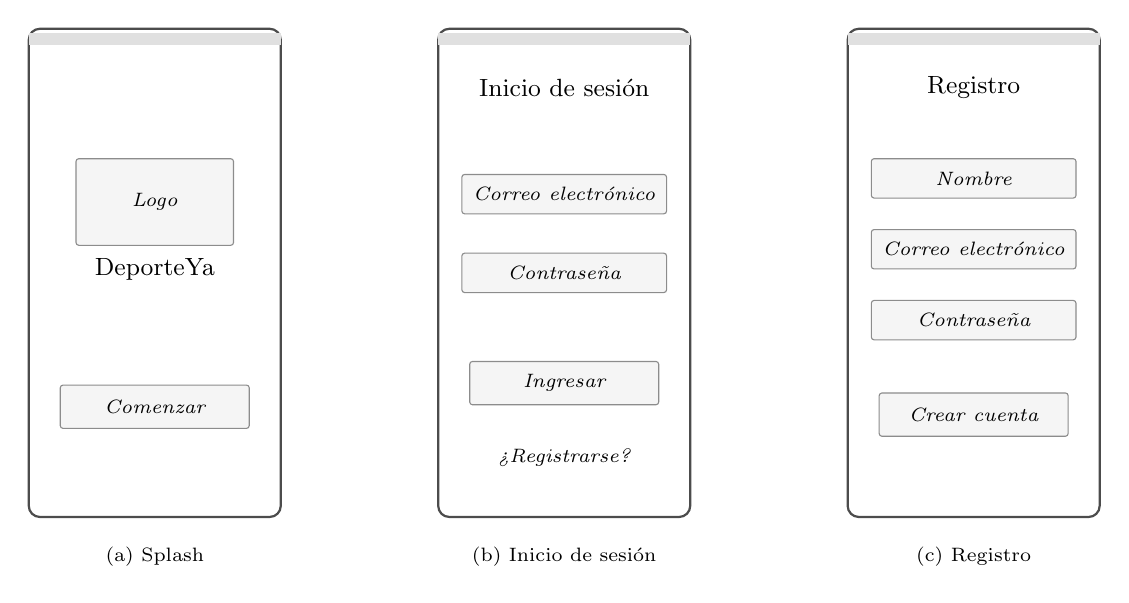
\begin{tikzpicture}[
      tel/.style={draw=black!70, thick, rounded corners=4pt, minimum width=3.2cm, minimum height=6.2cm},
      zona/.style={draw=black!45, thin, rounded corners=1pt, fill=gray!8},
      etiqueta/.style={font=\scriptsize\itshape, align=center},
      etqPantalla/.style={font=\scriptsize, align=center}
    ]
    % --- (a) Splash ---
    \begin{scope}[xshift=0cm]
      \node[tel] (a1) at (0,0) {};
      \fill[black!12] (-1.6,2.9) rectangle (1.6,3.05);
      \node[zona, minimum width=2.0cm, minimum height=1.1cm] at (0,0.9) {};
      \node[etiqueta] at (0,0.9) {Logo};
      \node[font=\small] at (0,0.05) {DeporteYa};
      \node[zona, minimum width=2.4cm, minimum height=0.55cm] at (0,-1.7) {};
      \node[etiqueta] at (0,-1.7) {Comenzar};
      \node[etqPantalla] at (0,-3.6) {(a) Splash};
    \end{scope}

    % --- (b) Inicio de sesión ---
    \begin{scope}[xshift=5.2cm]
      \node[tel] (b1) at (0,0) {};
      \fill[black!12] (-1.6,2.9) rectangle (1.6,3.05);
      \node[font=\small] at (0,2.35) {Inicio de sesi\'on};
      \node[zona, minimum width=2.6cm, minimum height=0.5cm] at (0,1.0) {};
      \node[etiqueta] at (0,1.0) {Correo electr\'onico};
      \node[zona, minimum width=2.6cm, minimum height=0.5cm] at (0,0.0) {};
      \node[etiqueta] at (0,0.0) {Contrase\~na};
      \node[zona, minimum width=2.4cm, minimum height=0.55cm] at (0,-1.4) {};
      \node[etiqueta] at (0,-1.4) {Ingresar};
      \node[etiqueta] at (0,-2.35) {¿Registrarse?};
      \node[etqPantalla] at (0,-3.6) {(b) Inicio de sesi\'on};
    \end{scope}

    % --- (c) Registro ---
    \begin{scope}[xshift=10.4cm]
      \node[tel] (c1) at (0,0) {};
      \fill[black!12] (-1.6,2.9) rectangle (1.6,3.05);
      \node[font=\small] at (0,2.35) {Registro};
      \node[zona, minimum width=2.6cm, minimum height=0.5cm] at (0,1.2) {};
      \node[etiqueta] at (0,1.2) {Nombre};
      \node[zona, minimum width=2.6cm, minimum height=0.5cm] at (0,0.3) {};
      \node[etiqueta] at (0,0.3) {Correo electr\'onico};
      \node[zona, minimum width=2.6cm, minimum height=0.5cm] at (0,-0.6) {};
      \node[etiqueta] at (0,-0.6) {Contrase\~na};
      \node[zona, minimum width=2.4cm, minimum height=0.55cm] at (0,-1.8) {};
      \node[etiqueta] at (0,-1.8) {Crear cuenta};
      \node[etqPantalla] at (0,-3.6) {(c) Registro};
    \end{scope}
  \end{tikzpicture}
  \caption{Wireframes de baja fidelidad de las pantallas de acceso}
\end{figure}

\begin{figure}[H]
  \centering
  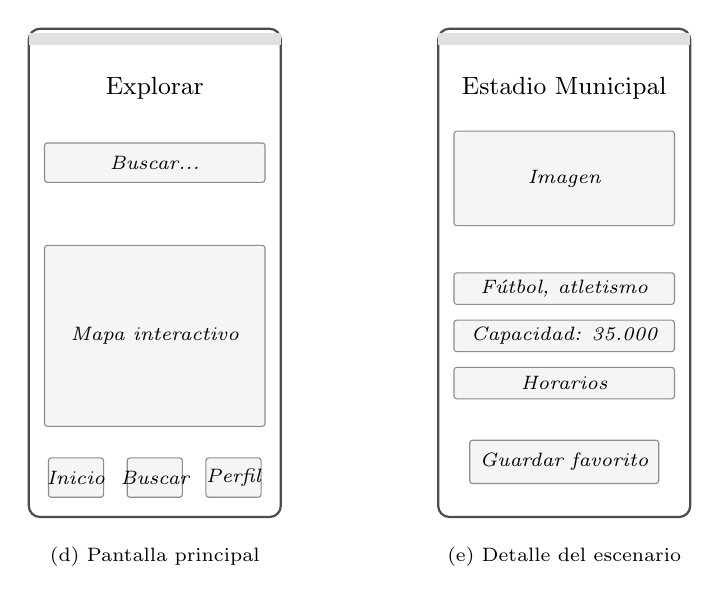
\begin{tikzpicture}[
      tel/.style={draw=black!70, thick, rounded corners=4pt, minimum width=3.2cm, minimum height=6.2cm},
      zona/.style={draw=black!45, thin, rounded corners=1pt, fill=gray!8},
      etiqueta/.style={font=\scriptsize\itshape, align=center},
      etqPantalla/.style={font=\scriptsize, align=center}
    ]
    % --- (d) Pantalla principal (mapa) ---
    \begin{scope}[xshift=0cm]
      \node[tel] (d1) at (0,0) {};
      \fill[black!12] (-1.6,2.9) rectangle (1.6,3.05);
      \node[font=\small] at (0,2.35) {Explorar};
      \node[zona, minimum width=2.8cm, minimum height=0.5cm] at (0,1.4) {};
      \node[etiqueta] at (0,1.4) {Buscar...};
      \node[zona, minimum width=2.8cm, minimum height=2.3cm] at (0,-0.8) {};
      \node[etiqueta] at (0,-0.8) {Mapa interactivo};
      \node[zona, minimum width=0.7cm, minimum height=0.5cm] at (-1.0,-2.6) {};
      \node[etiqueta] at (-1.0,-2.6) {Inicio};
      \node[zona, minimum width=0.7cm, minimum height=0.5cm] at (0,-2.6) {};
      \node[etiqueta] at (0,-2.6) {Buscar};
      \node[zona, minimum width=0.7cm, minimum height=0.5cm] at (1.0,-2.6) {};
      \node[etiqueta] at (1.0,-2.6) {Perfil};
      \node[etqPantalla] at (0,-3.6) {(d) Pantalla principal};
    \end{scope}

    % --- (e) Detalle del escenario ---
    \begin{scope}[xshift=5.2cm]
      \node[tel] (e1) at (0,0) {};
      \fill[black!12] (-1.6,2.9) rectangle (1.6,3.05);
      \node[font=\small] at (0,2.35) {Estadio Municipal};
      \node[zona, minimum width=2.8cm, minimum height=1.2cm] at (0,1.2) {};
      \node[etiqueta] at (0,1.2) {Imagen};
      \node[zona, minimum width=2.8cm, minimum height=0.4cm] at (0,-0.2) {};
      \node[etiqueta] at (0,-0.2) {F\'utbol, atletismo};
      \node[zona, minimum width=2.8cm, minimum height=0.4cm] at (0,-0.8) {};
      \node[etiqueta] at (0,-0.8) {Capacidad: 35.000};
      \node[zona, minimum width=2.8cm, minimum height=0.4cm] at (0,-1.4) {};
      \node[etiqueta] at (0,-1.4) {Horarios};
      \node[zona, minimum width=2.4cm, minimum height=0.55cm] at (0,-2.4) {};
      \node[etiqueta] at (0,-2.4) {Guardar favorito};
      \node[etqPantalla] at (0,-3.6) {(e) Detalle del escenario};
    \end{scope}
  \end{tikzpicture}
  \caption{Wireframes de baja fidelidad de las pantallas principales}
\end{figure}

% ============================================================================
%  SECCIÓN 3.8: TECNOLOGÍAS PRELIMINARES
% ============================================================================

\section{Tecnolog\'ias preliminares}

Para el desarrollo de la aplicaci\'on m\'ovil se propone un conjunto de
tecnolog\'ias de c\'odigo abierto y de amplia adopci\'on, que permiten construir
una soluci\'on multiplataforma con un \'unico c\'odigo base y reducir los costos y
tiempos de desarrollo \citep{pressman2010}. En la tabla se presentan las
tecnolog\'ias propuestas para cada componente del sistema; estas podr\'an
ajustarse en los siguientes avances de acuerdo con las necesidades del
proyecto.

\begin{table}[H]
  \centering
  \caption{Tecnolog\'ias preliminares del proyecto}
  \contenidoConFuente{%
    \begin{tablaAPA}
      \begin{tabular}{@{}p{2.8cm}p{4.6cm}p{8.2cm}@{}}
        \toprule
        \textbf{Capa} & \textbf{Tecnolog\'ia} & \textbf{Justificaci\'on} \\
        \midrule
        Frontend m\'ovil & React Native + Expo &
        Desarrollo multiplataforma (iOS y Android) con un \'unico c\'odigo base;
        Expo simplifica la compilaci\'on y la publicaci\'on \citep{reactnative,
        expo}. \\
        \addlinespace
        Mapas y georreferenciaci\'on & Leaflet &
        Librer\'ia de c\'odigo abierto para mapas interactivos, ligera y
        compatible con dispositivos m\'oviles \citep{leaflet, longley2015}. \\
        \addlinespace
        Backend & Node.js + Express &
        Mismo lenguaje que el frontend m\'ovil, alto rendimiento y amplia
        comunidad de desarrollo \citep{nodejs}. \\
        \addlinespace
        Base de datos & PostgreSQL + PostGIS &
        Base de datos relacional confiable con extensi\'on espacial para
        consultas geogr\'aficas sobre la ubicaci\'on de los escenarios
        \citep{postgresql}. \\
        \addlinespace
        Backend como servicio & Supabase &
        Autenticaci\'on, base de datos y almacenamiento integrados, con plan
        gratuito adecuado para el proyecto \citep{supabase}. \\
        \addlinespace
        Control de versiones & Git + GitHub &
        Colaboraci\'on del equipo y trazabilidad de los cambios en el c\'odigo. \\
        \bottomrule
      \end{tabular}
    \end{tablaAPA}%
  }{Elaboraci\'on propia en base a la revisi\'on documental.}
\end{table}

En cuanto al dise\~no de la interfaz, los wireframes de baja fidelidad se
realizaron directamente como diagramas esquem\'aticos (secci\'on de wireframes
iniciales) y la interfaz de la aplicaci\'on se construye y valida directamente
sobre el c\'odigo con React Native, verificando el resultado mediante capturas
de la aplicaci\'on ejecutada en el dispositivo f\'isico.


% --- Referencias (APA) ------------------------------------------------------
\newpage
\bibliographystyle{apacite}
\nocite{*}
\bibliography{formato/referencias}

% --- Anexos (material complementario, tras las referencias) ------------------
\newpage
\appendix
% ============================================================================
%  ANEXO A: CRONOGRAMA DE ACTIVIDADES
% ============================================================================

\section{Anexo A: Cronograma de actividades}

El siguiente cronograma presenta las fases y actividades principales del
proyecto, distribuidas a lo largo de la gesti\'on acad\'emica. Las semanas son
referenciales y pueden ajustarse seg\'un el calendario de la asignatura.

\begin{table}[H]
  \centering
  \caption{Cronograma de actividades del proyecto}
  \begin{tablaAPA}
    \begin{tabular}{@{}p{3.6cm}p{8.2cm}p{3.2cm}@{}}
      \toprule
      \textbf{Fase} & \textbf{Actividades principales} & \textbf{Semanas} \\
      \midrule
      An\'alisis & Identificaci\'on de la problem\'atica, revisi\'on de
      antecedentes, levantamiento de requerimientos y definici\'on de usuarios. &
      Semanas 1--3 \\
      \addlinespace
      Dise\~no & Wireframes, flujo de navegaci\'on, arquitectura del sistema y
      modelo de datos. & Semanas 4--6 \\
      \addlinespace
      Desarrollo & Configuraci\'on del entorno, desarrollo del backend y base de
      datos, e implementaci\'on del frontend web y m\'ovil. & Semanas 7--11 \\
      \addlinespace
      Pruebas & Pruebas funcionales, de usabilidad y de rendimiento; correcci\'on
      de errores. & Semanas 12--13 \\
      \addlinespace
      Cierre & Documentaci\'on final, preparaci\'on de la presentaci\'on y
      entrega del producto. & Semanas 14--16 \\
      \bottomrule
    \end{tabular}
  \end{tablaAPA}
\end{table}

\section{Anexo B: Casos de uso}
% TODO: Diagramas y descripciones de los principales casos de uso.

% ============================================================================
%  ANEXO C: MODELO DE DATOS
% ============================================================================

\section{Anexo C: Modelo de datos}

El modelo de datos propuesto para el sistema est\'a conformado por las
siguientes entidades principales, dise\~nadas para almacenar la informaci\'on de
los escenarios deportivos y las interacciones de los usuarios. La base de
datos utilizar\'a PostgreSQL con la extensi\'on espacial PostGIS para gestionar
las coordenadas de ubicaci\'on de cada escenario \citep{postgresql}.

\begin{table}[H]
  \centering
  \caption{Entidades del modelo de datos}
  \begin{tablaAPA}
    \begin{tabular}{@{}p{2.8cm}p{5.6cm}p{7.2cm}@{}}
      \toprule
      \textbf{Entidad} & \textbf{Descripci\'on} & \textbf{Atributos principales} \\
      \midrule
      Usuario & Persona que utiliza el sistema & id, nombre, correo,
      contrase\~na, rol, fecha\_registro \\
      \addlinespace
      Escenario & Escenario deportivo registrado & id, nombre, tipo,
      descripci\'on, capacidad, direcci\'on, latitud, longitud, estado \\
      \addlinespace
      Deporte & Disciplina deportiva & id, nombre, descripci\'on \\
      \addlinespace
      Evento & Evento programado en un escenario & id, escenario\_id, nombre,
      fecha, hora, descripci\'on \\
      \addlinespace
      Imagen & Fotograf\'ia de un escenario & id, escenario\_id, url, orden \\
      \addlinespace
      Favorito & Relaci\'on entre usuario y escenario & id, usuario\_id,
      escenario\_id, fecha \\
      \addlinespace
      Valoraci\'on & Opini\'on de un usuario sobre un escenario & id,
      usuario\_id, escenario\_id, puntuaci\'on, comentario, fecha \\
      \bottomrule
    \end{tabular}
  \end{tablaAPA}
\end{table}

Las relaciones principales entre las entidades son las siguientes: un usuario
puede registrar varios favoritos y valoraciones, y un escenario puede recibir
favoritos y valoraciones de distintos usuarios (relaciones uno a muchos); un
escenario puede albergar varios deportes y un deporte puede practicarse en
varios escenarios (relaci\'on muchos a muchos); y un escenario puede tener
varios eventos e im\'agenes asociadas (relaciones uno a muchos).

\section{Anexo D: Presupuesto}
% TODO: Detallar costos estimados (infraestructura, licencias, recursos humanos).

% ============================================================================
%  ANEXO E: ENCUESTA AL PÚBLICO
% ============================================================================

\section{Anexo E: Encuesta al p\'ublico}

El siguiente cuestionario se aplicar\'a al p\'ublico general para diagnosticar
el acceso a la informaci\'on deportiva y conocer los requerimientos de la
aplicaci\'on m\'ovil de visualizaci\'on interactiva de escenarios deportivos.

\textbf{Instrucciones:} marque con una X la opci\'on que mejor refleje su
situaci\'on.

\begin{enumerate}
  \item \textquestiondown Con qu\'e frecuencia practica deporte o asiste a
        eventos deportivos (f\'utbol, baloncesto, voleibol, atletismo, etc.)?
        \begin{itemize}
          \item[$\square$] Semanalmente
          \item[$\square$] Mensualmente
          \item[$\square$] Trimestralmente
          \item[$\square$] Rara vez
        \end{itemize}

  \item \textquestiondown C\'omo se entera habitualmente de la oferta
        deportiva de su ciudad (escenarios, horarios y eventos)?
        \begin{itemize}
          \item[$\square$] Redes sociales
          \item[$\square$] Carteles y volantes
          \item[$\square$] Recomendaciones de conocidos
          \item[$\square$] P\'aginas web o aplicaciones
        \end{itemize}

  \item \textquestiondown Encuentra f\'acilmente la informaci\'on sobre los
        escenarios deportivos de su regi\'on?
        \begin{itemize}
          \item[$\square$] S\'i, siempre
          \item[$\square$] A veces
          \item[$\square$] No, casi nunca
        \end{itemize}

  \item \textquestiondown Qu\'e informaci\'on considera m\'as importante al
        buscar un escenario deportivo? (puede marcar m\'as de una)
        \begin{itemize}
          \item[$\square$] Ubicaci\'on y mapa
          \item[$\square$] Disciplinas y capacidad
          \item[$\square$] Horarios y eventos programados
          \item[$\square$] Servicios disponibles
        \end{itemize}

  \item \textquestiondown Utilizar\'ia una aplicaci\'on m\'ovil que
        permita visualizar en un mapa interactivo todos los escenarios
        deportivos del pa\'is?
        \begin{itemize}
          \item[$\square$] S\'i, definitivamente
          \item[$\square$] Probablemente s\'i
          \item[$\square$] Probablemente no
          \item[$\square$] No
        \end{itemize}
\end{enumerate}

\textbf{FUENTE:} Elaboraci\'on propia.

% ============================================================================
%  ANEXO F: GUÍA DE ENTREVISTA A GESTORES DE ESCENARIOS
% ============================================================================

\section{Anexo F: Gu\'ia de entrevista a gestores de escenarios deportivos}

La siguiente gu\'ia orienta las entrevistas semiestructuradas que se
realizar\'an a los gestores de los escenarios deportivos seleccionados en el
piloto.

\begin{enumerate}
  \item \textquestiondown Cu\'al es la trayectoria y la actividad principal del
        escenario deportivo que usted gestiona?
  \item \textquestiondown Qu\'e disciplinas deportivas alberga el escenario y
        cu\'al es su capacidad aproximada?
  \item \textquestiondown Qu\'e medios utiliza actualmente para difundir los
        horarios, los servicios y los eventos del escenario?
  \item \textquestiondown Considera que la difusi\'on de su escenario llega
        adecuadamente al p\'ublico? \textquestiondown Por qu\'e?
  \item \textquestiondown Qu\'e informaci\'on de su escenario considera esencial
        que la poblaci\'on conozca (ubicaci\'on, capacidad, accesibilidad,
        servicios)?
  \item \textquestiondown Ha utilizado alguna plataforma digital para difundir
        su oferta deportiva? \textquestiondown Con qu\'e resultados?
  \item \textquestiondown Estar\'ia dispuesto a registrar la informaci\'on de su
        escenario en un sistema nacional de visualizaci\'on interactiva?
  \item \textquestiondown Qu\'e beneficios y dificultades prev\'e en la
        utilizaci\'on de este tipo de plataforma?
\end{enumerate}

\textbf{FUENTE:} Elaboraci\'on propia.


\end{document}
